
% !TeX spellcheck = en_US
%	TODO	-	Outlier beschreiben 
 
\section{Results}

	%------------------------------%
	%& 			In General 			
	%------------------------------%

		%------------------------------%
		%& 		Konvergenz				
		%------------------------------%
	
		CCA and db-RDA successfully ran for all models, while GLM$_{mv}$s and CAO/CQO had convergence problems. 
		%
		They mostly occurred with class four methods, which have a low sample size to parameter ratio (see Table \ref{table:classes}). 
		%
		For GLM$_{mv}$s non-convergence was determined by run time. 
		%
		Models that ran more than 18 hours were aborted and classified as non-converging.
		% 
		Non-convergence of GLM$_{mv}$s occurred for all class four and one class two (Uni-Uni) model. 
		%
		CAO failed to converge for all level four models of \textit{Uni-Li} and \textit{Uni-Bi}; CQO for  all class four models of \textit{Uni-Bi}, for unequal and identity tolerance models of \textit{Uni-Uni} and for unequal tolerance models of \textit{Uni-Lo, Lo-Bi} and \textit{Bi-Bi}.\\

		%------------------------------%
		%& 		Runtime 				
		%------------------------------% 
	
		$GLM_{mv}$ was the slowest method. 
		%
		For a class three \textit{Uni-Uni} model the GLM$_{mv}$ ANOVA ran 03:13 h;
		db-RDA 1.7 min for axis and 4 s for terms; 
		CCA 2 s for axis and $< 1s $ for terms; 
		CAO 9 min  and in COQ 28 s for equal tolerance, 9 s for unequal tolerance and 6 s for identity tolerance (on an Ubuntu 18.04 machine with 64-bit, 8 GB RAM and 1.6 GHz).

		%------------------------------%
		%& 		Verweise 				
		%------------------------------%  
	
		Means and standard deviations of \textit{p}-values of GLM$_{mv}$, db-RDA and CCA for all covariables are shown in Table \ref{table:results1}.
		
		I refer to the Supplementary Materials for tables of covariable and axes \textit{p}-values at the level of response combinations or classes (Table \ref{tab:SMGLM1} - \ref{tab:ccasm4}), CCA inertias (Table \ref{tab:smcca5} and \ref{tab:smcca6}), Canonical Coefficients of CAO (Table \ref{tab:caosm1} and \ref{tab:caosm2}) and CQO (Table \ref{tab:cqosm1} - \ref{tab:cqosm3}) as well as selected ordination diagramms (Figures \ref{fig:smdbord} - \ref{fig:smcqoord}).
		
		%------------------------------%
		%& Tabelle: p-Werte + Standard Deviations
		%------------------------------% 
		
		\begin{table*}[h!]
			\centering
			\caption{\textit{p}-values $\pm$ standard deviations of the variables and axes from GLM$_{mv}$, db-RDA and CCA for all models. Not included are CAO and CQO as they do not provide \textit{p}-values. The categories Axes1-3+ do not apply to GLM$_{mv}$ as they do not use latent axes. Axis3+ denotes all axes from the third upwards. }	
				\begin{tabular}{@{}cccc@{}}
					\toprule
								   & \textbf{GLM$_{mv}$}               & \textbf{db-RDA}		    & \textbf{CCA} \\
					\hline
					\textit{env1}  & \small $0.002\ \pm\ 0,001$ & \small $0.001\ \pm\ 0.001$ & \small $0.201\ \pm\ 0.401$ \\
					\textit{env2}  & \small $0.003\ \pm\ 0.002$ & \small $0.015\ \pm\ 0.006$ & \small $0.101\ \pm\ 0.003$ \\
					\textit{Noise} & \small $0.579\ \pm\ 0.270$ & \small $0.471\ \pm\ 0.257$ & \small $0.353\ \pm\ 0.309$ \\
					\textit{Axis1} & 			NA				& \small $0.002\ \pm\ 0.003$ &	\small $0.001\ \pm\ 0.000$ \\	
					\textit{Axis2} & 			NA				& \small $0.061\ \pm\ 0.176$ &  \small $0.146\ \pm\ 0.279$ \\
					\textit{Axis3+}&			NA				& \small $0.604\ \pm\ 0.279$ & \small  $0.738\ \pm\ 0.374$ \\
					\bottomrule
				\end{tabular}
				
				\label{table:results1}	
		\end{table*}

	%------------------------------%
	%& 		GLMmv 					
	%------------------------------%
	
	\subsection{Multivariate Generalized Linear Models}
	
		%------------------------------%
		%& 			In General 			
		%------------------------------%
		In the GLM$_{mv}$s, most models had their lowest AIC and did not violate assumptions with a negative binomial residual distributions.
		% TODO What patterns? Violate what assumption ? 
		Only in \textit{Li-Li}, \textit{Li-Lo} and \textit{Lo-Lo} was the assumption that residuals are independent of predictors violated, as they showed arched patterns in their residual plots.  
		%
		Based on better fit in the QQ-Plot, a negative binomial distribution was used in \textit{Li-Li} and \textit{Lo-Lo} and a normal distribution in \textit{Li-Lo}.
		
		%------------------------------%
		%& 		multivaritate p-values 	
		%------------------------------% 
		
		GLM$_{mv}$'s multivariate \textit{p}-values for both environmental variables, all classes and response type combinations were very low.
		%
		The \textit{p}-values for noise variables were higher and more spread.
		%
		The standard deviation of noise variable \textit{p}-values was higher in linear and logistic responses (0.306) than in unimodal and bimodal ones (0.187).
		%
		The \textit{p}-values of noise variables only fell below the nominal significance level of 0.05 in six models (three form \textit{Li-Bi} and \textit{Lo-Lo} each).  
		%
		For \textit{env1} there was no clear difference between model classes. 
		%
		In \textit{env2}, additional samples decreased the mean \textit{p}-value from 0.003 to 0.002, while also decreasing standard deviation from 0.002 to 0.001. 
		%
		Adding noise variables increased their mean \textit{p}-value from 0.41 to 0.57. 
		%
		Adding samples further increased it to 0.62. (see Table \ref{tab:SMGLM1} in Supplementary Materials)\\

		%------------------------------%
		%& 		univariate p-values 	
		%------------------------------% 

		Univariate \textit{p}-values were high if a species had its optimum in the middle of an uni- or bimodal gradient (cf. Figure \ref{fig:hohep}).
		%
		Exceptions were \textit{Lo-Bi} and \textit{Li-Bi}, in which both environmental gradients had low \textit{p}-values for all species.
		%
		In \textit{Bi-Bi}, \textit{Uni-Li} and \textit{Uni-Lo} the high \textit{p}-values for the first environmental variable were separated into two groups. 
		%
		In all three cases the lower \textit{p}-values were associated with class three models and hence increased sample size.
		%
		In \textit{Uni-Lo}, species one to three had higher \textit{p}-values than the remaining species for the logistic gradient (see Figure \ref{fig:hohep}).
		%
		Other than that, both environmental gradients received low \textit{p}-values for all species.
		%
		Due to the problems with intermediate uni- or bimodal species, the mean \textit{p}-values for \textit{env1} and \textit{env2} were high: 0.158$\ \pm$ 0.34 and 0.134 $\ \pm\ $ 0.32. 
		%
		When these species are not considered the means drop to 0.003 $\pm$ 0.004 and 0.004 $\pm$ 0.004. \\
		%
		The mean of noise variable \textit{p}-values was 0.80 $\pm$ 0.24. 
		%
		Adding noise variables and increasing sampling size both lowered the \textit{p}-values of environmental gradients and increased those of noise variables. The smallest noise variable \textit{p}-values mostly (25 of 29 below 0.05) originated form class three models. 
		
		%Figure Unimodal and bimodal \textit{p}-values in GLM species test 
		%------------------------------%
		%& Figure: Unimodal p-values in uni and bimodal GLM	
		%------------------------------% 
		\begin{figure}[h!]
			\centering
			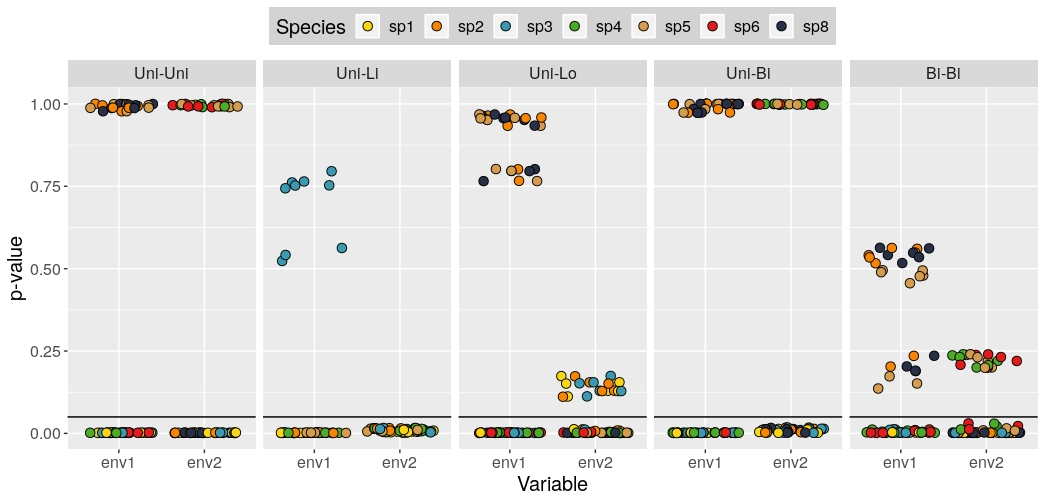
\includegraphics[width=0.9\linewidth]{../02_Figures/01_GLMmv/glm_uni_hohep}
			\caption{
				Univariate GLM$_{mv}$ \textit{p}-values of models containing unimodal or bimodal response types, except \textit{Lo-Bi} and \textit{Li-Bi}. Species that have their optimum at the center of a gradient show higher \textit{p}-values on the corresponding variable. 
				The black line indicates a \textit{p}-value of 0.05. Species identity is indicated via point color.
				Species 7 and 9 are not shown, as their \textit{p}-values did not show any pattern.
				}
			\label{fig:hohep}
		\end{figure}


	%------------------------------%
	%& 	db-RDA 	
	%------------------------------% 
	\subsection{Distance Based Redundancy Analysis}

		db-RDA assigned low \textit{p}-values to most environmental variables.
		%
		Environmental variables only received high \textit{p}-values in \textit{Uni-Li} and \textit{Uni-Lo}, where higher \textit{p}-values were associated with the non-unimodal gradient and class four models.
		%
		For both environmental variables mean \textit{p}-values and standard deviations were highest in class four models. 
		%
		The lowest mean \textit{p}-values for noise variables occurred in \textit{Lo-Lo} at $0.383\ \pm\ 0.206$. 
		%
		\textit{Bi-Bi} had the most noise variable \textit{p}-values below 0.05 and was the only model including one in a class one model. 
		%
		Class three models had the lowest mean \textit{p}-value for noise variables ($Mean\ \pm\ SD\ \scriptscriptstyle Noise,\ class\ 3 \textstyle = 0.431\ \pm\ 0.238$) and class four the highest ($Mean\ \pm\ SD\ \scriptscriptstyle Noise,\ class\ 4  \textstyle = 0.506\ \pm\ 0.289$).\\
		%
		Mean \textit{p}-values for the first constrained axis were low, while for the second they were higher and more spread. 
		%
		For all response types and model classes, environmental variables load stronger on the first two constrained axes than the noise variables.
		%
		The third and higher constrained axes were mostly structured by noise variables and had high \textit{p}-values. 
		%
		The second axis had higher \textit{p}-values in class four models ($Mean\ \pm\ SD\ \scriptscriptstyle CAP2,\ Class\ 4 \textstyle = 0.240\ \pm\ 0.288$)
		than in the other classes ($Mean\ \pm\ SD\ \scriptscriptstyle CAP2,\ Class\ 1,2,3 \textstyle = 0.003\ \pm\ 0.002$).
		%
		This effect is strongest in models with linear or logistic responses.
		%

		%------------------------------%
		%& 	Plot 4: CCA vs. db-RDA p-values 	
		%------------------------------% 
		
		% TODO Graif anders erwähnen
		%Figure \ref{fig:p-compare} shows the \textit{p}-values for \textit{env1} and \textit{env2} as well as the  noise-variables from all models of db-RDA and CCA.
	
	% Figure CCA vs db-RDA p-values.
		\begin{figure}[h!]
			\centering
			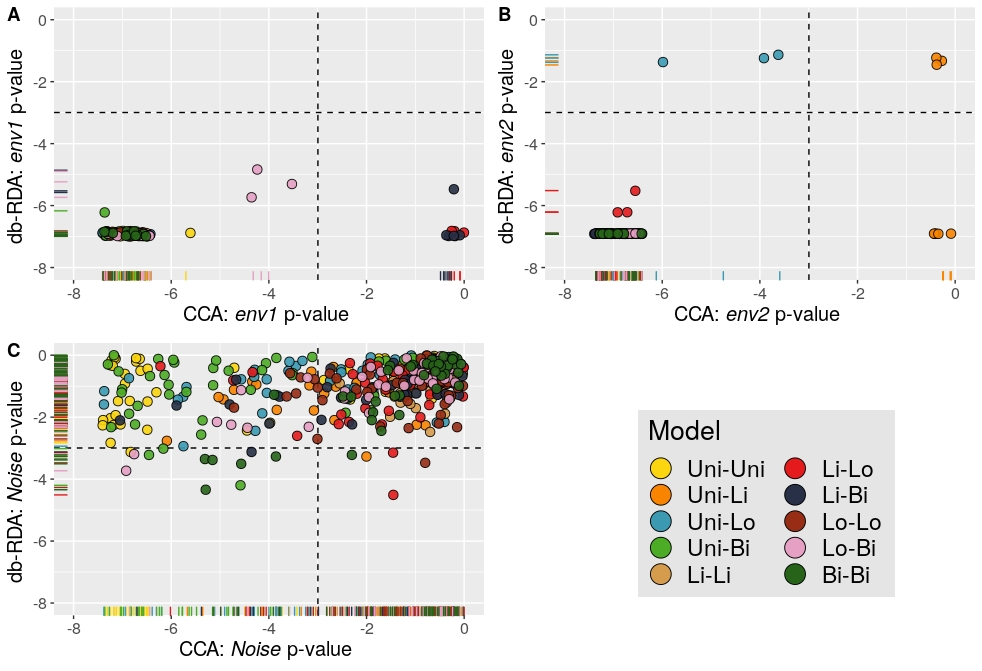
\includegraphics[width=1\linewidth]{../02_Figures/P-Compare}
			\caption{
				\textit{p}-values of (\textbf{a}) \textit{env1},   (\textbf{b}) \textit{env2} and (\textbf{c}) \textit{noise variables} for db-RDA and CCA. Y- and X-axis are scaled with a natural logarithm. Black lines indicated \textit{p}-values of 0.05. Rugs and points are jittered. The color of the points corresponds to the response type combination. 
			}
			\label{fig:p-compare}
		\end{figure}

	%------------------------------%
	%& 			CCA					
	%------------------------------% 

	\subsection{Canonical Correspondence Analysis}

		%------------------------------%
		%& 			Variablen			
		%------------------------------% 
		CCA assigned high \textit{p}-values to linear gradients if only one of the gradients was linear.
		%
		In \textit{Li-Li}, both gradients received low \textit{p}-values.
		%
		Accordingly, mean \textit{p}-values for \textit{env1} and \textit{env2} are high and wide spread. 
		%
		The \textit{p}-values for noise variables were low in comparison to the other methods.
		%
		Leaving out the three models with one linear response (\textit{Uni-Li}, \textit{Li-Lo} and \textit{Li-Bi}), decreased \textit{p}-values of \textit{env1} and \textit{env2} $(Mean\ \pm\ SD\ \scriptscriptstyle env1\ \&\  env2\ \textstyle = 0.001\ \pm\ 0.003$), while the mean \textit{p}-value for noise variables remained at 0.34 $\pm$ 0.32.\\
		%
		Noise \textit{p}-values were especially low in \textit{Uni-Uni} ($Mean\ \pm\ SD = 0.155 \pm\ 0.251$) and \textit{Uni-Bi} ($Mean\ \pm\ SD = 0.118\ \pm\ 0.193$). 
		%
		Noise variable \textit{p}-values in \textit{Bi-Bi} were markedly higher ($Mean\ \pm\ SD = 0.507\ \pm\ 0.336$). \\
		%
		The different classes did not have an impact on \textit{env1} and \textit{env2}. 
		%
		In noise variables the \textit{p}-value decreased when additional noise variables were added and increased with increasing sample sizes. \\
	
		%------------------------------%
		%& 			Axes			
		%------------------------------% 
		The first CCA axis had very low \textit{p}-values, independent of response type or class ($Mean\ \pm\ SD\ \scriptscriptstyle CCA1 \textstyle < 0.001\ \pm\ 0$). 
		%
		For the response combinations \textit{Uni-Li}, \textit{Li-Lo} and \textit{Li-Bi} the second axis had high \textit{p}-values ($Mean\ \pm\ SD\ =  0.459\ \pm\ 0.336$), but was also strongly determined by noise variables.
		%
		Overall, the mean \textit{p}-value for the second axis was higher than for the first.
		%
		Removing the three models \textit{Uni-Li, Li-Lo} and \textit{Li-Bi} reduced its \textit{p}-value to 0.011 $\pm$ 0.055. 
		%
		In \textit{Lo-Bi}, the second axis had considerably higher \textit{p}-values in the class four models 
		($Mean\ \pm\ SD\ \scriptscriptstyle Lo-Bi,\ class 4 \textstyle = 0.260\ \pm\ 0.170$)
		than in the other three classes  
		($Mean\ \pm\ SD\ \scriptscriptstyle Lo-Bi,\ class\ 1,2,3 \textstyle = 0.001\ \pm\ < 0.001$). 
		%
		In all response types, the axes three and higher were determined strongest by noise variables and \textit{p}-values were high. 
		%
		\textit{Uni-Uni} and \textit{Uni-Bi} had low \textit{p}-values for the third and higher axes: 
		$Mean\ \pm\ SD\ \scriptscriptstyle CCA3+, Uni-Uni \textstyle = 0.364\ \pm\ 0.416$;
		$Mean\ \pm\ SD\ \scriptscriptstyle CCA3+, Uni-Bi  \textstyle = 0.407\ \pm\ 0.407$.\\
		
		%------------------------------%
		%& 			Inertia				
		%------------------------------% 
		
		Total inertia differed between response types: Uni- and bimodal responses had the highest total inertia ($Mean\ \pm\ SD\ \scriptscriptstyle Uni/Bi-X \textstyle = 4.45\ \pm\ 1.94$), linear and logistic the lowest ($Mean\ \pm\ SD\ \scriptscriptstyle Li/Lo-X \textstyle = 0.15\ \pm\ 0.13$). 
		%
		Mixtures of these response types lay in between ($Mean\ \pm\ SD\ \scriptscriptstyle Li/Lo-Uni/Bi\textstyle = 1.60\ \pm\ 0.80$).
		%
		This pattern was also found in constrained and unconstrained inertia (see Supplementary Materials Table \ref{tab:ccasm2}).

	%------------------------------%
	%& 			CAO/ CQO			
	%------------------------------% 
	
	\subsection{Constrained Additive and Quadratic Ordination}
	
	%------------------------------%
	%& 	Parameter estimation		
	%------------------------------% 	
	
		For	models with only linear or logistic responses, i.e. \textit{Li-Li, Li-Lo} and \textit{Lo-Lo}, CAO failed to estimate any species parameters. 
		%
		Its also in these models and in \textit{Bi-Bi}, that both variables contributed equally to the latent variable. 
		%
		In the others, one variable determined the latent gradient while the other contributed as much as the noise variables (see Figure \ref{fig:caoonlyone}). 
		%
		\textit{Uni-Lo} was the only response combination for which all parameters were estimated in all classes. 
		%
		In all other combinations, CAO failed to estimate at least some parameters.
		%
		In \textit{Uni-Bi} and \textit{Uni-Uni} estimation failed only for class four models.
		
	%------------------------------%
	%& 	Species Maxima				
	%------------------------------%	
		Species maxima were underestimated for every response combination. 
		%
		The mean difference between estimated and actual maxima, expressed in percent of actual maxima was $-84.9\ \%\ \pm\ 9.3$ \%.\\ 
	
	%------------------------------%
	%& 	Figure: CAO loadings		
	%------------------------------%	
	\begin{figure}[h!]
		\centering
		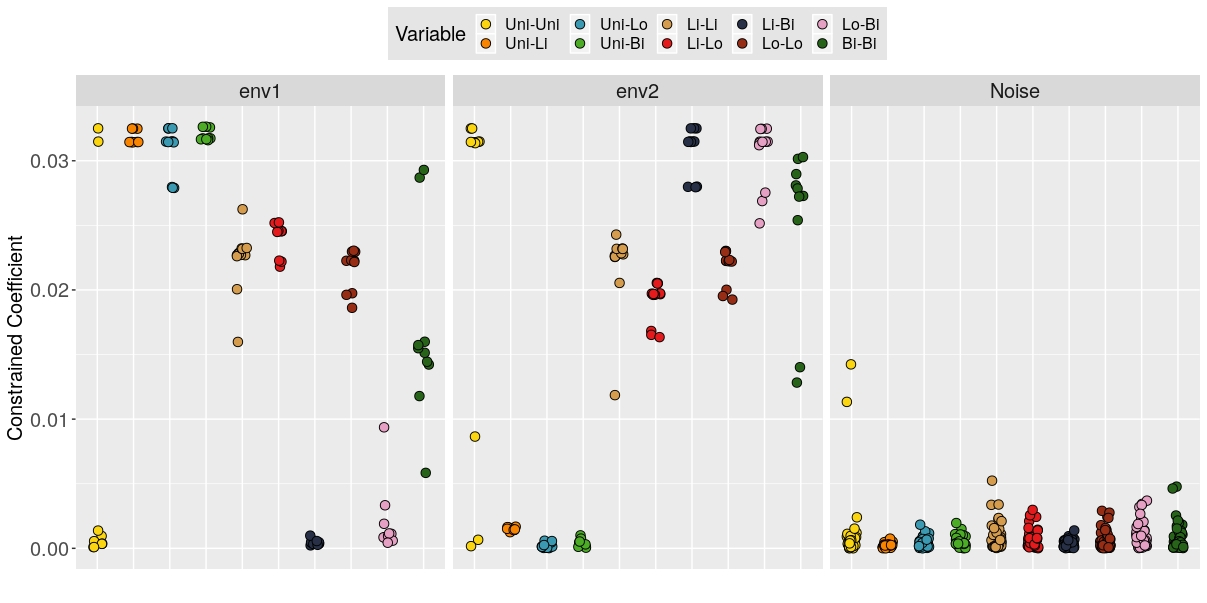
\includegraphics[width=1\linewidth]{../02_Figures/02_CAO/CAO_loadings}
		\caption{
			Absolute values of constrained coefficients from the Constrained Additive Ordination. 
			%
			Colors indicate the response type combination. 
			%
			Each box contains the values for one covariable. 
			%
			Points are horizontally jittered.
		}
		\label{fig:caoonlyone}
	\end{figure}
	%


	%------------------------------%
	%& 			CQO					
	%------------------------------%
	
	Constrained coefficients did not differ significantly between tolerance types, but varied strongly among response types (see Figure \ref{fig:cqoweights}).
	%
	The weights of uni- or bimodal responses were higher than those of logistic or linear ones. 
	%
	The bimodal gradient in class four, unequal tolerance \textit{Li-Bi} (0.277) had the highest coefficient and the linear gradient in the same model the lowest (0.001).
	%
	The weight of a gradient depended not only on the response type but also on the other gradient.
	%
	For example, the mean coefficient of the unimodal gradient in \textit{Uni-Uni} is 0.18, while it is 0.09 in \textit{Uni-Li}. 
	%
	The mean weights for \textit{env1} and \textit{env2} were $0.079\ \pm\ 0.062$ and $0.064\ \pm\ 0.049$. 
	%
	Outliers are often results of class four models, for example, in \textit{Uni-Uni} and \textit{Li-Bi}. 
	%
	However, in some models (e.g. \textit{Uni-Bi}) outliers were generated by other model classes. 

	Overall, the weights of noise variables were markedly lower than those of environmental variables ($Mean\ \pm\ SD_{\scriptscriptstyle Noise} = 0.002\ \pm\ 0.003$).  
	%
	The coefficient was highest in \textit{Uni-Uni} with 0.006 and lowest in \textit{Lo-Lo} with 0.001.
	%
	More noise variables and fewer samples increased the weights of noise variables and decreased those of environmental variables. 
	%
	Additional samples had the opposite effect. \\
	
	There was no overarching effect of either class or tolerance assumption on constrained coefficients. 
	%
	The only notable effect was the lower convergence rate of unequal tolerance models.
	%
	The estimated maxima were extremely inaccurate. 
	%
	In most cases, they were too high, but occasionally also too small. 
	%
	An illustrative example is the equal tolerance, class three, \textit{Uni-Bi} model: For two seeds the maximum abundance of species 9 was overestimated by 1.7e+98 \% of the actual maximum and for the other seed it was underestimated by 100 \%. 
	
	\begin{figure}[h!]
		\centering
		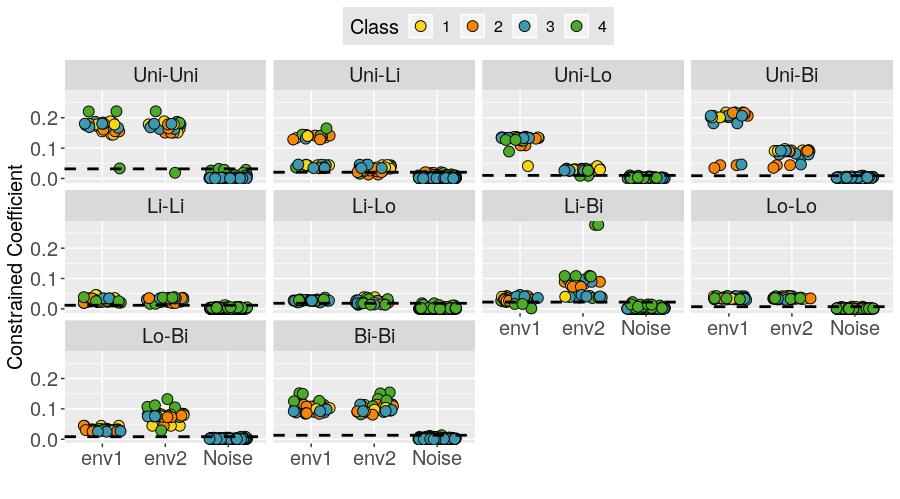
\includegraphics[width=1\linewidth]{../02_Figures/02_CAO/CQOPlotalsJpg}
		\caption{Constrained Coefficients of explanatory variables in a Constrained Quadratic Ordination. Each box is one response type combination. Point colors indicate the model class. The black line marks the highest weight of a noise variable for that response type combination. The points are horizontally jittered. }
		\label{fig:cqoweights}
	\end{figure}
















